%%%%%%%%%%%%%%%%%%%%%%%%%%%%%%%%%%%%%%%%%%%%%%%%%%%%%%%%%%%%
% 源文件排版规范:
% chapter分文件放置于子目录下,需要clearpage
% section前空三行
% subsection前空两行
% subsubsection及以下级别前空一行
%%%%%%%%%%%%%%%%%%%%%%%%%%%%%%%%%%%%%%%%%%%%%%%%%%%%%%%%%%%%
\documentclass[10pt]{article}
\usepackage{xeCJK}                      % xeCJK
\usepackage{fontspec}                   % 字体选择
\usepackage{fontenc}                    % 字体选择
\usepackage{cite}                       % 引用
\usepackage{natbib}                     % Bibtex引用
\usepackage{indentfirst}                % 首行缩进
\usepackage{hyperref}                   % 目录链接
\usepackage{geometry}                   % 页面调整
\usepackage{chemfig}                    % 化学
\usepackage[version=4]{mhchem}          % 化学
%\usepackage{amsmath}                   % 数学
%\usepackage{amssymb}                   % 数学
%\usepackage{calc}                      % 数学
\usepackage{siunitx}                    % 表格
\usepackage{supertabular}               % 超级表格
\usepackage{multirow}                   % 合并单元格
%%%%%%%%%%%%%%%%%%%%%%%%%%%%%%%%%%%%%%%%%%%%%%%%%%%%%%%%%%%%
\geometry{                              % 页面调整B5活页纸
	dvipdfm,
	left=2.1cm,
	right=2.1cm,
	top=1cm,
	bottom=1.5cm,
	body={14cm,20cm},
	papersize={18.2cm,22.5cm}
}
\hypersetup{                            % 链接颜色调整
    colorlinks,
    citecolor=black,
    filecolor=black,
    linkcolor=black,
    urlcolor=black
}
\setCJKmainfont{Hiragino Sans GB}       % 中文字体
\setmainfont{Times New Roman}           % 西文字体
\XeTeXlinebreaklocale "zh"              % 中文自动换行
\XeTeXlinebreakskip = 0pt plus 1pt
\setlength{\parindent}{2em}             % 首行缩进
\linespread{1.2}                        % 行间距
\setlength{\parskip}{0.5\baselineskip}  % 段间距
\renewcommand\arraystretch{1.5}         % 表格高度调整
\setcounter{tocdepth}{3}                % 目录深度(打印设为1)
%%%%%%%%%%%%%%%%%%%%%%%%%%%%%%%%%%%%%%%%%%%%%%%%%%%%%%%%%%%%
\renewcommand\contentsname{目录}
\renewcommand\bibname{参考文献}
\title{化学实验}
\author{胡译文}
\date{}
%%%%%%%%%%%%%%%%%%%%%%%%%%%%%%%%%%%%%%%%%%%%%%%%%%%%%%%%%%%%
\begin{document}
	\maketitle
	\tableofcontents
	
	
	\clearpage
	\section{基本仪器}
	
	
	\subsection{容器}
	\begin{itemize}
		\item 直接加热:
		\begin{itemize}
			\item 试管:倾斜 $\ang{45}$ ,加热时液体不超过 $1/3$
			\item 坩锅:在泥三角上加热,用坩埚钳夹取。用于熔化、加热、反应等。瓷坩锅含 \ce{SiO2}。
			\item 蒸发皿:玻璃棒搅拌,用 坩埚钳夹取
		\end{itemize}
		\item 隔网加热:
		\begin{itemize}
			\item 烧杯(加热时液体不超过 $1/2$ 的容积)
			\item 烧瓶:圆底烧瓶(盛装液体占 $1/3$ 至 $2/3$ 的容积)、蒸馏烧瓶、平底烧瓶
			\item 锥形瓶(盛装液体不超过 $1/2$ 的容积)
			\item 三颈烧瓶
		\end{itemize}
		\item 不能加热:集气瓶、表面皿
	\end{itemize}
	
	
	\subsection{量器}
	\begin{itemize}
		\item 粗量仪器:托盘天平、量筒(平视凹液面最低处)、温度计
		\item 精量仪器:容量瓶、滴定管
	\end{itemize}
	
	\subsubsection{温度计}
	
	温度计使用时注意量程、不能碰壁。
	
	\paragraph{测反应混合物的温度}
	
	将温度计插入混合物中间。
	
	\begin{itemize}
		\item 测物质溶解度、实验室制乙烯
	\end{itemize}
	
	\paragraph{测蒸气的温度}
	
	由于液体沸腾时,液体和蒸气的温度相同,所以只要测蒸气的温度。
	
	\begin{itemize}
		\item 实验室蒸馏石油、测定乙醇的沸点
	\end{itemize}
	
	\paragraph{测水浴温度}
	
	要使反应物的温度保持相对稳定,所以恒温水浴加热,温度计则插入水浴中。
	
	\begin{itemize}
		\item 温度对反应速率影响的反应、中和热的测定、苯的硝化反应、实验室制乙烯、蒸馏
	\end{itemize}
	
	\subsubsection{容量瓶}
	\paragraph{使用方法}
	\begin{enumerate}
		\item \textbf{检漏:}加水,塞好瓶塞,倒立,瓶塞周围无水漏出,将瓶正立并将瓶塞旋转$\ang{180}$后塞紧,再倒立,无水漏出
		\item \textbf{计算}
		\item \textbf{称量(天平、药匙)或量取(量筒)}
		\item \textbf{溶解或稀释:}在烧杯中加适量水溶解或稀释,玻璃棒搅拌,冷却。
		\item \textbf{移液:}玻璃棒引流
		\item \textbf{洗涤:}洗涤烧杯,洗涤液也转移到容量瓶内, 次。
		\item \textbf{定容:}先玻璃棒引流加水至刻度线下$1\text{--}2cm$处,然后用胶头滴管滴加至平视凹液面最低处与刻度线相平
		\item \textbf{摇匀:}左手顶在瓶塞,右手五指轻托平底,反复颠倒上下摇匀
	\end{enumerate}
	\paragraph{注意事项}
	\begin{itemize}
		\item 不能在容量瓶里进行溶质的溶解,应将溶质在烧杯中溶解、冷却后转移
		\item 溶液不能超过容量瓶的标线,一旦超过,必须重新进行配制
		\item 容量瓶不能进行加热
		\item 选用时需要标明规格($1/2.5/5\times 10^n mL$)
	\end{itemize}
	
	\subsubsection{滴定管}
	滴定管度数上小下大。
	\begin{itemize}
		\item 酸式滴定管(玻璃旋钮):不能用于碱性物质
		\item 碱式滴定管(橡胶管):不能用于强氧化性物质和有机溶剂
	\end{itemize}
	
	
	\subsection{分离仪器}
	
	\begin{itemize}
		\item 固液分离:普通漏斗
		\item 液液分离:分液漏斗
		\item 气气分离:洗气瓶、干燥管
	\end{itemize}
	
	\subsubsection{干燥管}
	
	\paragraph{种类}
	球形干燥管(盛装固体干燥剂)、U形干燥管(盛装液体或固体干燥剂)

	\paragraph{常见干燥剂}
	
	\begin{itemize}
		\item 浓 \ce{H2SO4}:酸性干燥剂,液体
		\item \ce{P2O5}固体:酸性干燥剂
		\item 碱石灰:碱性干燥剂
		\item 无水 \ce{CaCl2}:中性干燥剂,不能干燥 \ce{NH3} (生成络合物)
		\item 无水 \ce{CuSO4}:中性干燥剂,万能干燥剂
		\item 无水 \ce{MgSO4}:中性干燥剂、有机干燥剂
		\item 无水 \ce{Na2SO4}:中性干燥剂、有机干燥剂
	\end{itemize}
	

	\subsection{其他}
	\begin{itemize}
		\item 玻璃棒、胶头滴管(不能:平放或倒置、碰壁、伸入容器)、冷凝管、水槽、铁架台
		\item 酒精灯(酒精需盛装 $1/4$ 至 $2/3$ 的容积)、酒精喷灯
	\end{itemize}
	
	\subsubsection{冷凝管}
	\begin{itemize}
		\item 直形冷凝管:必须斜用或平用
		\item 球形冷凝管:可以竖用,用于冷凝回流一般气体
		\item 蛇形冷凝管:一般竖用,用于冷凝回流沸点很低的有机物或冷 凝有毒气体
	\end{itemize}
	
	\subsubsection{启普发生器}
	
	\paragraph{构造}
	
	启普发生器由三部分构成:球型漏斗、容器部分、带活塞的导管部分。
	
	\paragraph{工作原理}
	
	以实验室制氢气为例,使用时,开启活塞,酸由球形漏斗流入容器至其与锌粒接触,反应产生氢气。关闭活塞,由于氢气压强增大,酸被压回球形漏斗,与锌粒脱离接触,反应停止。
	
	\paragraph{使用条件}
	
	固液不加热制取气体、反应不剧烈、块状固体、气体不能太溶于水

	\paragraph{气密性检验}
	
	关闭导气管上的活塞,从球形漏斗口处加入水,当水浸没球形漏斗下端后,继续加入水,球形漏斗内外会出现液面差,观察液面,在一段时间内不发生变化,表明气密性良好。
	
	\paragraph{常见反应}
	
	\begin{itemize}
		\item \ce{HCl}和 \ce{FeS}制取 \ce{H2S}
		\item \ce{HCl}和 \ce{CaCO3}制取 \ce{CO2}
		\item \ce{H2SO4}和金属制取 \ce{H2}
		\item 其余反应均\textbf{不能}用启普发生器
	\end{itemize}
	
	
	\subsection{总结}
	
	\subsubsection{特殊仪器}
	
	\paragraph{需要验漏的仪器}
	
	容量瓶、分液漏斗、滴定管
	
	\paragraph{需要标注规格的仪器}
	
	量筒、容量瓶
	
	\paragraph{玻璃仪器}
	
	(各种)漏斗、酒精灯、温度计、水槽、启普发生器、(各种)杯/瓶/管、玻璃棒
	
	
	
	\clearpage
	\section{化学实验安全与试剂保存}
	
	
	\subsection{试剂保存}
	
	\subsubsection{试剂瓶的选择}
	
	\begin{itemize}
		\item 固体:广口瓶
		\item 液体:细口瓶
		\item 气体:集气瓶
		\item 光解:棕色瓶(碘、硝酸银 、溴化银、浓硝酸 、稀硝酸、氯水、溴水、碘水、银氨溶液)
		\item 玻璃塞:不能用于碱性物质
		\item 橡胶塞:不能用于强氧化性物质和有机溶剂
	\end{itemize}
	
	\subsubsection{危险标志}
	
	\begin{center}
		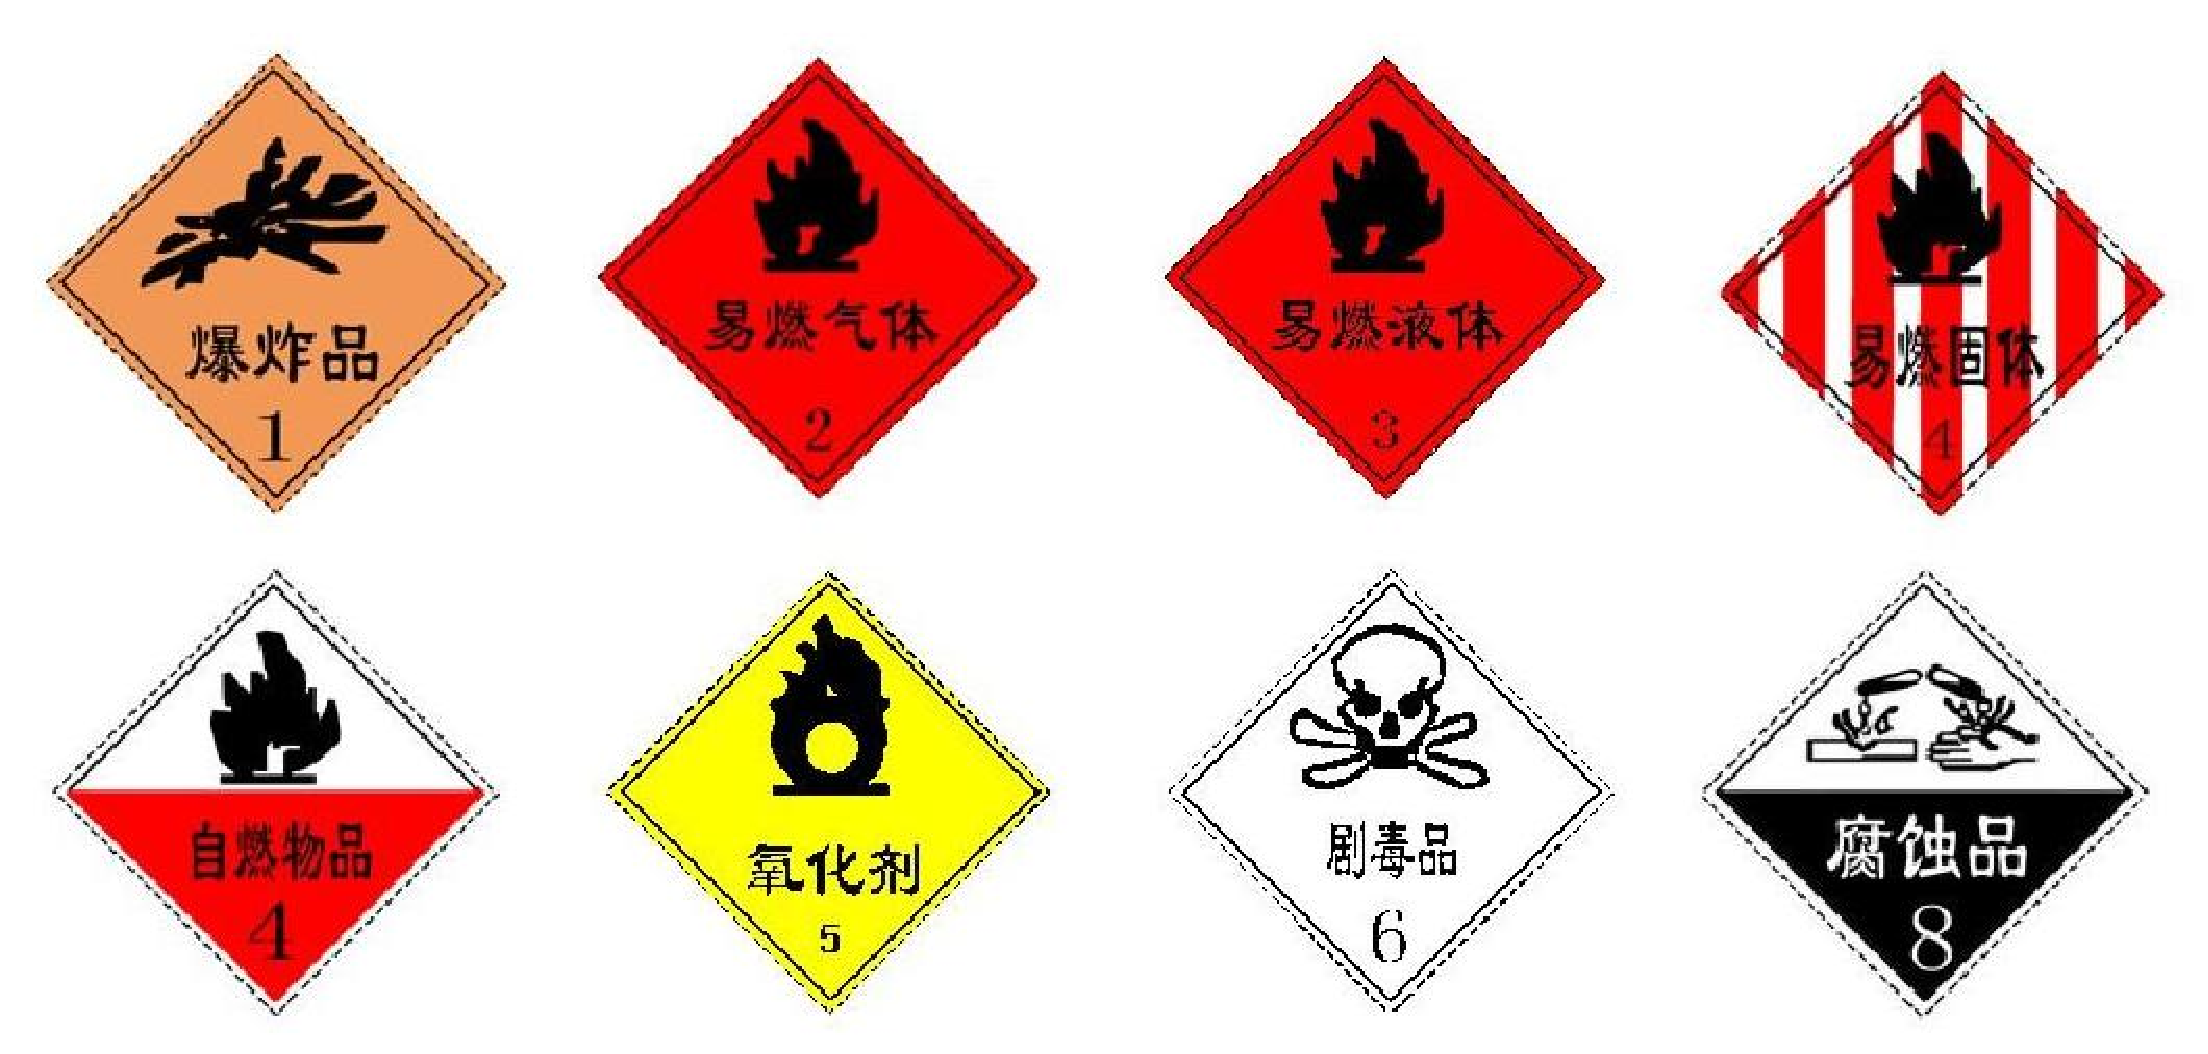
\includegraphics[scale=0.38]{res/hazard}
	\end{center}
	
	\subsubsection{一些试剂保存方式}
	
	\begin{itemize}
		\item 氢氟酸:不能放在玻璃容器内,应该放在塑料容器内避光保存。
		\item 镁:无需保存于煤油中,因为会形成氧化膜保护。
	\end{itemize}
	
	
	\subsection{事故处理}
	
	化学实验中常见事故的处理:
	
	\begin{center}
	\tablefirsthead{
		\hline
		\multicolumn{2}{|c|}{\textbf{意外事故}} & \textbf{处理方法} \\}
	\tablehead{
		\hline
		\multicolumn{3}{|l|}{\small\sl 接上页}\\\hline
		\multicolumn{2}{|c|}{\textbf{意外事故}} & \textbf{处理方法} \\}
	\tabletail{
		\hline
		\multicolumn{3}{|r|}{\small\sl 接下页}\\
		\hline}
	\tablelasttail{\hline}
	
	\begin{supertabular}{|m{2cm}<{ \centering}|m{3cm}<{ \centering}|m{9cm}<{ \centering}|}
		\hline
		\multicolumn{2}{|c|}{酒精及其他易燃有机物小面积失火} & 立即用湿布或沙土扑盖 \\ \hline
		\multicolumn{2}{|c|}{钠、磷等失火} & 迅速用沙子覆盖 \\ \hline
		
		腐蚀性酸 & \multirow{2}{=}{ \centering 流到桌子上} & 用适量 \ce{NaHCO3}冲洗,后用水冲洗 \\ \cline{1-1} \cline{3-3}
		腐蚀性碱 & ~ & 用适量稀醋酸冲洗,后用水冲洗 \\ \hline
		
		腐蚀性酸 & \multirow{2}{=}{ \centering 沾到皮肤上} & 用水冲洗,再用 \ce{NaHCO3}冲洗 \\ \cline{1-1} \cline{3-3}
		腐蚀性碱 & ~ & 用水冲洗,再用硼酸溶液冲洗 \\ \hline
		
		\multicolumn{2}{|c|}{腐蚀性酸、碱溅到眼中} & 用水反复冲洗,不断眨眼,后就医。不要用手揉眼睛。 \\ \hline
		\multicolumn{2}{|c|}{苯酚溅至皮肤} & 用酒精浸洗 \\ \hline
		\multicolumn{2}{|c|}{误食重金属盐} & 应立即口服生蛋清或牛奶 \\ \hline
		\multicolumn{2}{|c|}{汞滴落在桌上或地上} & 尽量回收,然后在桌子或地上撒上硫粉 \\
	\end{supertabular}
	\end{center}
	
	
	
	\clearpage
	\section{基本操作}
	
	\subsection{仪器的洗涤}
	
	使用毛刷,用去污剂和水冲洗。洗净标准:玻璃仪器内壁附着均匀的水膜,既不聚成水滴,也不成股流下。
	
	\subsubsection{洗涤试剂的选择}
	
	\begin{center}
	\tablefirsthead{
		\hline
		\textbf{残留物} & \textbf{洗涤剂} \\}
	\tablehead{
		\hline
		\multicolumn{2}{|l|}{\small\sl 接上页}\\\hline
		\textbf{残留物} & \textbf{洗涤剂} \\
		}
	\tabletail{
		\hline
		\multicolumn{2}{|r|}{\small\sl 接下页}\\
		\hline}
	\tablelasttail{\hline}
	\begin{supertabular}{|m{0.5\textwidth}<{ \centering}|m{0.5\textwidth}<{ \centering}|}
		\hline
		容器里附有的油污 & 热的碱性溶液 \\ \hline
		容器壁上附着的硫 & \ce{CS2}或热的 \ce{NaOH}溶液 \\ \hline
		试管壁上的银镜 & 稀硝酸 \\ \hline
		制 \ce{Cl2}时残留的 \ce{MnO2} & 热浓盐酸 \\
	\end{supertabular}
	\end{center}
	
	\subsection{装置气密性检查}
	
	装置气密性检查应在药品填装之前。

	$$
	\text{封闭}\rightarrow\text{改变内外压强(微热、加水等)}\rightarrow\text{描述现象(气泡、液面变化等)}\rightarrow\text{说明气密性良好}
	$$
	
	\subsubsection{常见方法}
	
	\begin{center}
		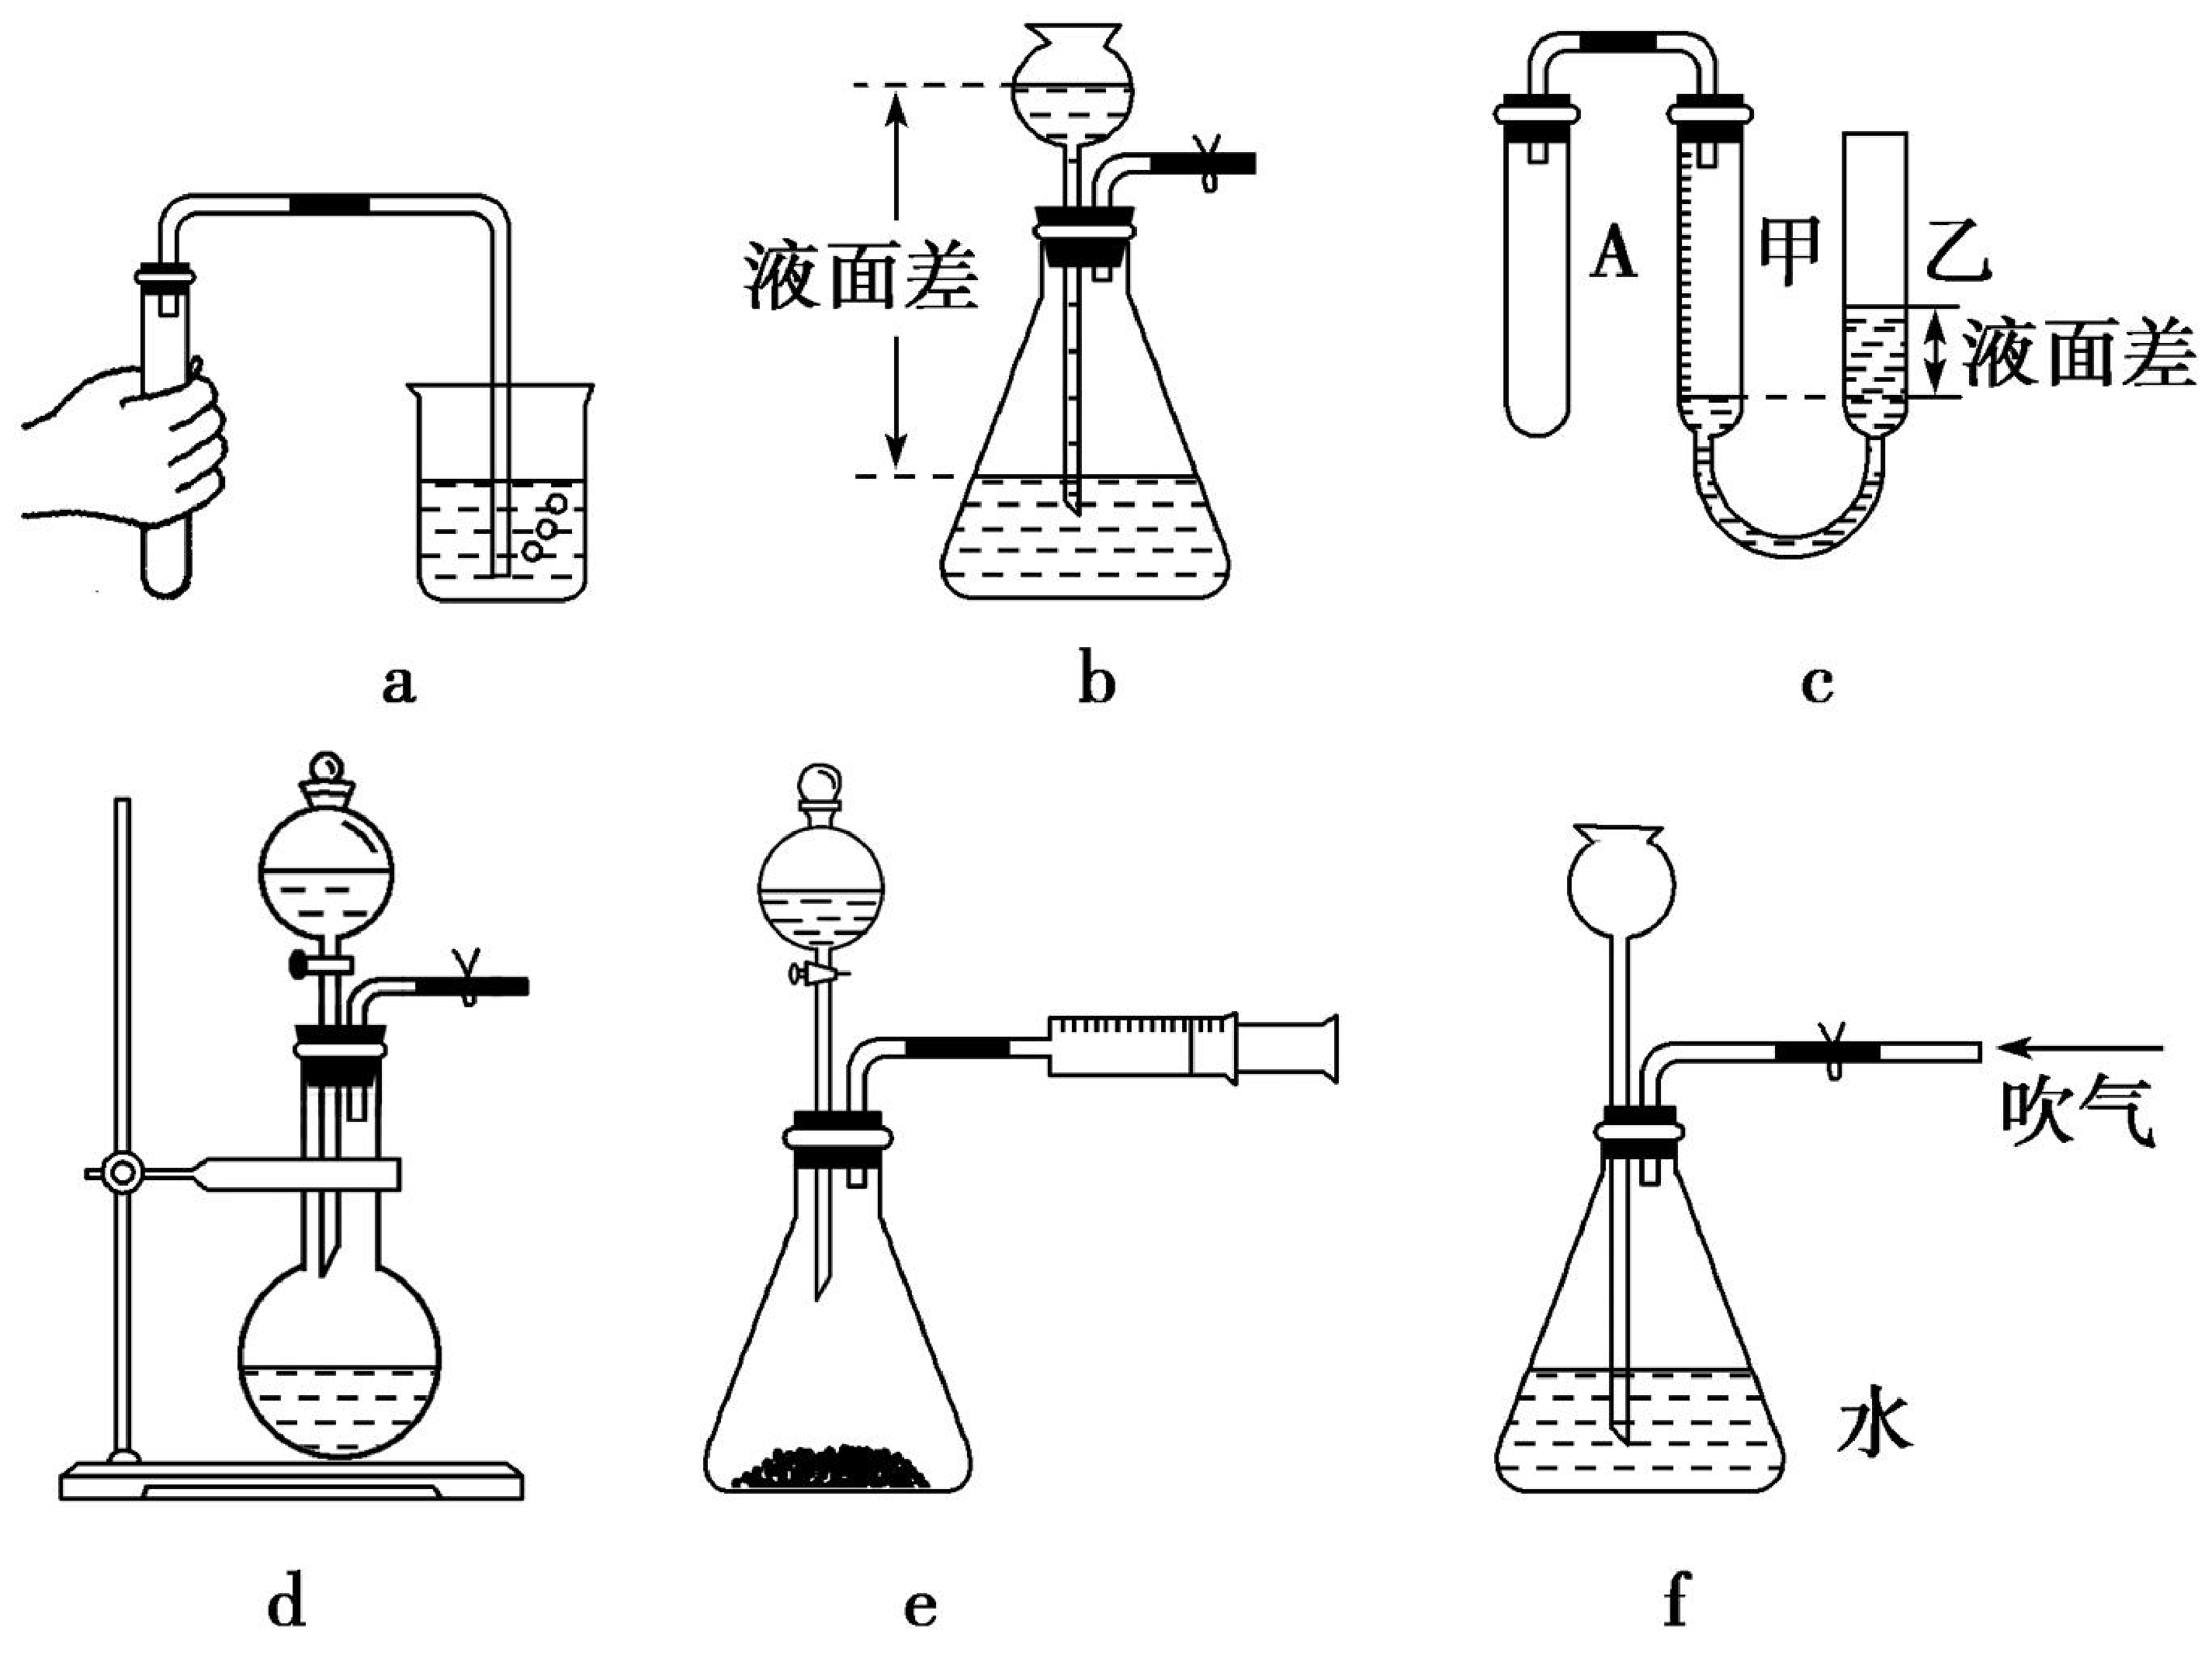
\includegraphics[scale=0.13]{res/airtight}
	\end{center}
		
	\paragraph{微热法}
	
	将导管插入盛装水的烧杯中,用酒精灯微热,导管口产生气泡,停止加热后导管内倒吸形成一段水柱,证明装置不漏气。
	
	$$
	\text{封闭}\rightarrow\text{微热}\rightarrow\text{观察气泡}\rightarrow\text{冷却导管中水柱上升}\rightarrow\text{说明气密性良好}
	$$
	
	\paragraph{液差法}
	
	夹紧弹簧夹,从长颈漏斗中注入适量水,使长颈漏斗液面高于锥形瓶液面,且保持不变,证明装置不漏气。
	
	$$
	\text{封闭}\rightarrow\text{加水形成液面高度差热}\rightarrow\text{停止加水}\rightarrow\text{观察液面不变化}\rightarrow\text{说明气密性良好}
	$$
	
	\paragraph{滴液法}
	
	向分液漏斗中注入适量水,关闭弹簧夹,打开分液漏斗活塞,如果水不能持续流下,则装置气密性良好。
	
	\paragraph{抽气法}
	
	关闭分液漏斗的活塞,轻轻向外拉动或向里推动注射器的活塞,一段时间后,活塞能回到原来的位置,表明装置的气密性良好。
	
	\paragraph{吹气法}
	
	打开弹簧夹,向导管口吹气,如果长颈漏斗中的液面上升,夹上弹簧夹且停止吹气后,长颈漏斗液面保持稳定,则表明装置的气密性良好。
	
	
	\subsection{试纸的使用}
	
	\subsubsection{常见类型}
	
	\begin{itemize}
		\item 石蕊试纸:
		\begin{itemize}
  			\item 红色石蕊试纸:用于检验碱性物质。
  			\item 蓝色石蕊试纸:用于检验酸性物质。
		\end{itemize}
		\item pH试纸:测量溶液的pH。
		\item 品红试纸:检验 \ce{SO2}等漂白性物质。
		\item 淀粉- \ce{KI}试纸:检验 \ce{Cl2}等氧化性的物质。
	\end{itemize}
	
	\subsubsection{使用方法}
	
	\begin{center}
	\tablefirsthead{
		\hline
		\textbf{所测物质} & \textbf{溶液} & \textbf{气体} & \textbf{pH值} \\}
	\tablehead{
		\hline
		\multicolumn{2}{|l|}{\small\sl 接上页}\\\hline
		\textbf{所测物质} & \textbf{溶液} & \textbf{气体} & \textbf{pH值} \\
		}
	\tabletail{
		\hline
		\multicolumn{4}{|r|}{\small\sl 接下页}\\
		\hline}
	\tablelasttail{\hline}
	\begin{supertabular}{|m{1.5cm}<{\centering}|m{4cm}<{\centering}|m{4cm}<{\centering}|m{4cm}<{\centering}|}
		\hline
		\multirow{2}{=}{ \centering 操作} & \multirow{2}{=}{ \centering 蘸取液体于试纸} & \multirow{2}{=}{ \centering \textbf{润湿}后置于气体中} & \multirow{2}{=}{ \centering 蘸取液体于试纸,与标准比色卡对照} \\
		~ & ~ & ~ & ~ \\ \hline
		注意 & \multicolumn{3}{c|}{无法检验 \ce{Cl2}、 \ce{HClO}溶液等,因为试纸会褪色。} \\ \hline
		润湿 &  & 必须润湿 & 不能润湿。(测得pH值:酸性溶液偏大,碱性溶液偏小,中性溶液不变。) \\
	\end{supertabular}
	\end{center}
	
	\paragraph{检验溶液}
	
	取一小块试纸放在玻璃片或表面皿上,用玻璃棒蘸取待测液体,点在试纸中部,观察试纸的颜色变化,确定溶液的性质。
	
	\paragraph{检验气体}
	
	先用蒸馏水把试纸润湿,用镊子夹取或粘在玻璃棒的一端,然后再放在集气瓶口或导管口处,观察试纸的颜色变化。
	
	\paragraph{pH试纸测定溶液pH值}	
	
	取一小块试纸放在玻璃片或表面皿上,用玻璃棒蘸取待测液体,点在试纸中部,观察试纸的颜色变化,与标准比色卡对照确定pH。
	
	\subparagraph{注意事项}
	
	\begin{itemize}
		\item 不能用蒸馏水润湿。(测得pH值:酸性溶液偏大,碱性溶液偏小,中性溶液不变。)
		\item 无法检验 \ce{Cl2}、 \ce{HClO}溶液等,因为试纸会褪色。
	\end{itemize}
	
	

	
	\subsection{药品的取用}
	
	\subsubsection{取用固体药品}
	
	\begin{itemize}
		\item 取用粉末状或小颗粒状固体,用药匙或纸槽,要把药品送入试管底部,而不能沾在管口和管壁上。
		\item 取用块状和大颗粒固体,用镊子夹取。
	\end{itemize}
	
	\subsubsection{取用液体药品}
	
	\begin{itemize}
		\item 取少量液体可用胶头滴管,取用较多的液体用倾倒法,注意试剂瓶上的标签朝向手心;向容量瓶、漏斗中倾倒液体时,要用玻璃棒引流。
	\end{itemize}
	
	\subsubsection{取用气体}
	
	难溶于水的气体可以如图所示进行储存和使用。
	
	\begin{center}
		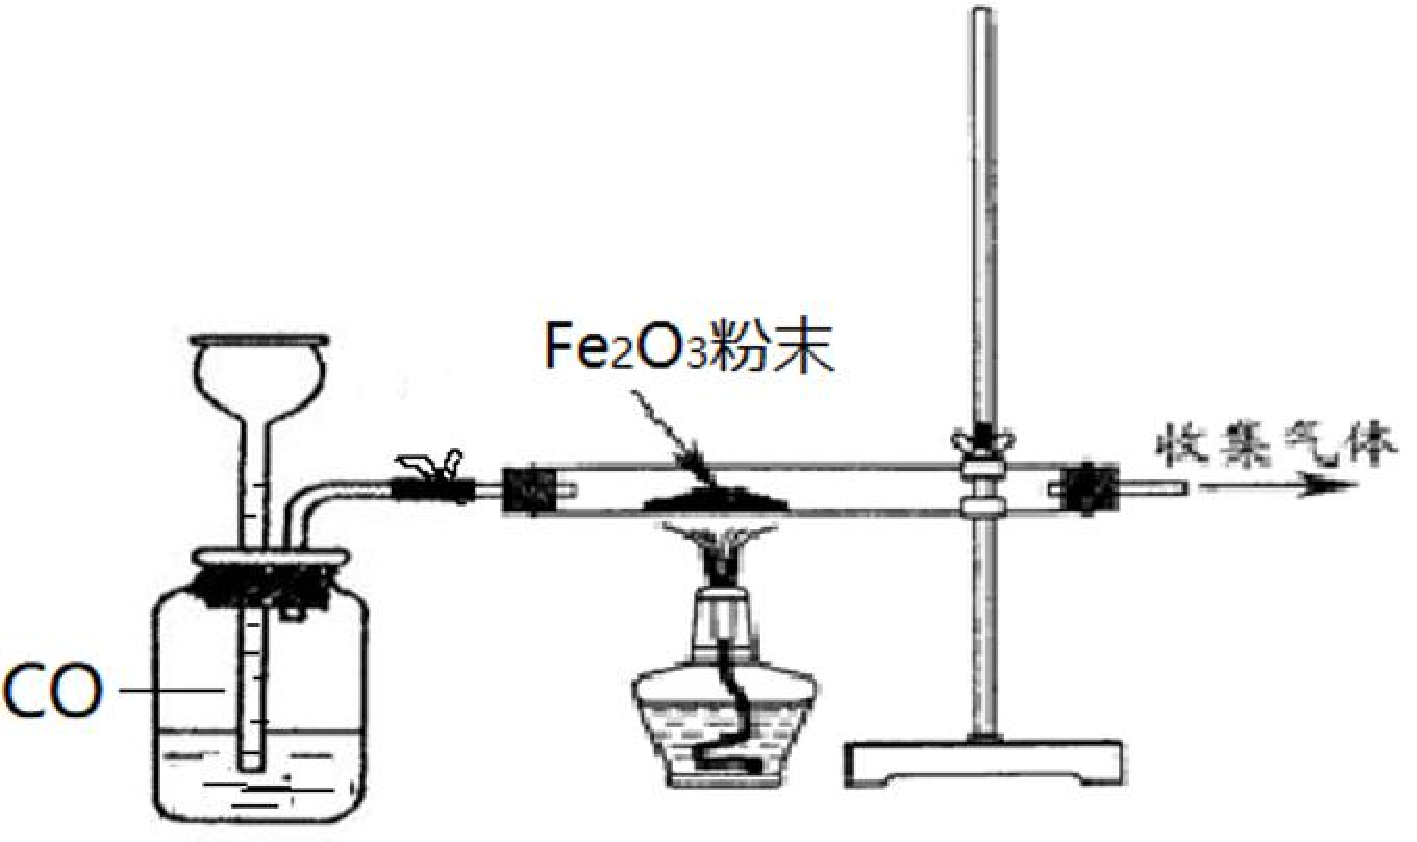
\includegraphics[scale=0.2]{res/gas.pdf}
	\end{center}
	
	
	\subsection{配置溶液}
	
	\subsubsection{固体物质的溶解}
	
	\begin{itemize}
		\item \underline{搅拌、震荡、加热}等措施可加快溶解速率。
		\item 一般将溶剂加入溶质中,但配制氯化铁、硫酸铝等一些易水解的盐溶液时,要将这些固体用相应酸溶解,再加入蒸馏水,以得到澄清溶液。
	\end{itemize}
	
	\subsubsection{液体物质的溶解}
	
	\begin{itemize}
		\item 一般把密度\textbf{大}的加入至密度\textbf{小}的液体中,如浓硫酸的稀释、浓硫酸与浓硝酸的混合等。
		\item 表述:将浓硫酸沿器壁缓缓注入水中,并同时用玻璃棒不断搅拌。
	\end{itemize}
	
	\subsubsection{气体的溶解}
	
	\paragraph{常见气体的溶解度($V_{\text{气体}}:V_{\text{液体}}$)}
	
	\begin{itemize}
		\item 难溶于水: \ce{H2}、 \ce{CO}、 \ce{CH4}、 \ce{N2}、 \ce{NO}。
		\item 微溶于水: \ce{O2}。
		\item 易溶于水: \ce{CO2}、 \ce{Cl2}、 \ce{H2S}、 \ce{SO2}($1:40$)、 \ce{HCl}($1:500$)、 \ce{NH3}($1:700$)。
	\end{itemize}
	
	\paragraph{装置选择}
	
	溶解度不大的气体,如CO2、Cl2、H2S等,可以直接通入水中;极易溶于水的气体,如 \ce{HCl}、 \ce{NH3}等,需要用防倒吸装置。
	
	
	\subsection{物质加热}
	
	比较不同的加热方式:
	
	\begin{center}
	\tablefirsthead{
		\hline
		\textbf{加热方式} & \multicolumn{2}{c|}{\textbf{适用范围或特点}} \\}
	\tablehead{
		\hline
		\multicolumn{3}{|l|}{\small\sl 接上页}\\\hline
		\textbf{加热方式} & \multicolumn{2}{c|}{\textbf{适用范围或特点}} \\
		}
	\tabletail{
		\hline
		\multicolumn{3}{|r|}{\small\sl 接下页}\\
		\hline}
	\tablelasttail{\hline}
	\begin{supertabular}{|m{3cm}<{ \centering}|m{6cm}<{ \centering}|m{3cm}<{ \centering}|}
		\hline
		直接加热 & \multicolumn{2}{c|}{瓷质、金属质或小而薄的玻璃仪器(如试管)等} \\ \hline
		隔石棉网加热 & \multicolumn{2}{c|}{较大的玻璃反应器(如烧杯、烧瓶等)} \\ \hline
		水浴 & \multirow{3}{=}{ \centering 反应器均匀受热且一定温度恒温加热} & $\SI{0}{ \celsius}$--$\SI{100}{ \celsius}$ \\ \cline{1-1} \cline{3-3}
		油浴 & ~ & $\SI{100}{ \celsius}$--$\SI{300}{ \celsius}$ \\ \cline{1-1} \cline{3-3}
		沙浴 & ~ & $\SI{300}{ \celsius}$--$\SI{500}{ \celsius}$ \\ \cline{1-1} \cline{3-3}
	\end{supertabular}
	\end{center}
	
	\subsubsection{固体的加热}
	
	\begin{itemize}
		\item 试管口要略向下倾斜,防止生成的水倒流,引起试管\textbf{炸裂}。
		\item 先给试管均匀加热,受热均匀后再固定在药品部位加热。
	\end{itemize}
	
	\subsubsection{液体的加热}
	
	\begin{itemize}
		\item 加热前,先把玻璃容器外壁的水擦干,以免炸裂试管;
		\item 用试管夹夹住试管中上部 $\frac 13$ 处,试管口擦干倾斜,不得对人,以防液体溅出烫伤。
	\end{itemize}
	
	
	\subsection{测定}
	
	\subsubsection{酸碱中和或氧化还原滴定}
	
	滴定管注意书写酸式还是碱式,读数精确到$0.01mL$。
	
	\paragraph{酸碱中和滴定指示剂变色pH值}
	
	\begin{center}
	\begin{tabular}{|m{2cm}<{ \centering}|m{2cm}<{ \centering}|m{1.5cm}<{ \centering}|m{2cm}<{ \centering}|m{1.5cm}<{ \centering}|m{2cm}<{ \centering}|m{1.5cm}<{ \centering}|}
		\hline
		\textbf{指示剂}  & \textbf{使用条件} & \textbf{颜色} & \textbf{临界pH值} & \textbf{颜色} & \textbf{临界pH值} & \textbf{颜色} \\ \hline
		石蕊 & 一般不使用 & 红 & $6$ & 紫 & $8$ & 蓝\\\hline
		甲基橙 & 终点酸性 & 红 & $3.1$ & 橙 & $4.4$ & 黄\\\hline
		酚酞 & 终点碱性 & 无 & $8.2$ & 浅红 & $10.0$ & 红\\\hline
	\end{tabular}
	\end{center}
	
	\paragraph{操作流程}
	
	\begin{itemize}
		\item \textbf{查:}(关闭滴定管活塞)装水至水零刻度线,直立静置不漏水(将旋钮旋转$\ang{180}$后再直立静置不漏水)。
		\item \textbf{洗: }洗净锥形瓶和滴定管,然后用标准液润洗滴定管 $2\text{--}3$ 次。
		\item \textbf{盛:}装入标准液,转动活塞快速放液(弯曲橡胶管挤压玻璃球),排除气泡。
		\item \textbf{调:}调节滴定管液面至 $0$ 刻度(或以下),记录读数。
		\item \textbf{滴定:}
		\begin{itemize}
			\item 左手:控制活塞;
			\item 右手:不断摇动锥形瓶;
			\item 眼睛:注视锥形瓶内溶液颜色及滴定流速.
		\end{itemize}
		\item \textbf{滴定终点:}滴入一滴标准液后,锥形瓶中发生变色,且半分钟内不恢复。
		\item \textbf{重复试验:} $3$ 次取平均值,要去掉差距特别大的数据。
	\end{itemize}
	
	\paragraph{氧化还原滴定指示剂}
	
	\begin{itemize}
		\item 高锰酸钾标准滴定溶液滴定产品草酸时,滴定终点为高锰酸钾标准滴定溶液的紫色。
		\item 碘量法滴定中,可溶性淀粉溶液和碘标准滴定溶液生成深蓝色。
	\end{itemize}
	
	\subsubsection{中和反应反应热测定}
	
	
	\clearpage
	\section{实验}
	
	\subsection{实验室气体制备}
	
	从左到右搭建实验装备,与大气联通。
	
	$$
	\text{发生装置} \rightarrow \text{净化装置} \rightarrow \text{干燥装置} \rightarrow \text{性质探究} \rightarrow \text{收集装置} \rightarrow \text{吸收装置}
	$$
	
	\subsubsection{常见气体的发生装置}
	
	
	\paragraph{固固加热型}
	
	\subparagraph{操作注意事项}
	
	\begin{itemize}
		\item 试管要干燥
		\item 试管口要略低于试管底
		\item 加热前要均匀预热
	\end{itemize}
	
	\paragraph{固液不加热和液液不加热型}
	
	\paragraph{启普发生器}
	
	见第一章。
	
	\paragraph{固液加热和液液加热型}
	
	\subparagraph{操作注意事项}
	
	\begin{itemize}
		\item 烧瓶加热时垫石棉网
		\item 反应物均为液体时要加沸石
	\end{itemize}
	
	\subsubsection{常见气体的制备}
	
	\begin{center}
	\tablefirsthead{
		\hline
		\textbf{气体} & \textbf{反应物} & \textbf{方程式} \\
		}
	\tablehead{
		\hline
		\multicolumn{3}{|l|}{\small\sl 接上页}\\\hline
		\textbf{气体} & \textbf{反应物} & \textbf{方程式} \\
		}
	\tabletail{
		\hline
		\multicolumn{3}{|r|}{\small\sl 接下页}\\
		\hline}
	\tablelasttail{\hline}
	\begin{supertabular}{|m{1cm}<{ \centering}|m{5cm}<{ \centering}|m{8cm}<{ \centering}|}
		\hline
		\multirow{3}{=}{ \centering \ce{O2}} & \ce{MnO2(s)}、 \ce{H2O2(aq)} & $ \ce{2H2O2 ->[MnO2] 2H2O + O2 ^}$ \\ \cline{2-3}
		~ & \ce{KClO3(s)}、 \ce{MnO2(s)} & $ \ce{2KClO3 ->[MnO2][\Delta] 2KCl + 3O2 ^}$ \\ \cline{2-3}
		~ & \ce{KMnO4(s)} & $ \ce{2KMnO4 ->[\Delta] K2MnO4 + MnO2 + 3O2 ^}$ \\ \hline
		\multirow{3}{=}{ \centering \ce{NH3}} & \ce{NH4Cl(s)}、 \ce{Ca(OH)2(s)} & $ \ce{2NH4Cl + Ca(OH)2 ->[\Delta] CaCl2 + 2NH3 ^ + 2H2O}$ \\ \cline{2-3}
		~ & \ce{CaO(s)}、浓 \ce{NH3*H2O} & $ \ce{NH3*H2O + CaO -> NH3 ^ + Ca(OH)2}$ \\ \cline{2-3}
		~ & \ce{NaOH(s)}、浓 \ce{NH3*H2O} & $ \ce{NH3*H2O ->[NaOH(s)] NH3 ^ + H2O}$ \\ \hline
		 \ce{CO2} & \ce{CaCO3(s)}、 \ce{HCl(aq)} & $ \ce{CaCO3 + 2HCl -> CaCl2 + H2O + CO2 ^}$ \\ \hline
		 \ce{H2} & \ce{Zn(s)}、 \ce{H2SO4(aq)}或 \ce{HCl(aq)} & $ \ce{Zn + H2SO4 -> ZnSO4 + H2 ^}$ \\ \hline
		 \ce{H2S} & \ce{FeS(s)}、 \ce{H2SO4(aq)}或 \ce{HCl(aq)} & $ \ce{FeS + H2SO4 -> FeSO4 + H2S ^}$ \\ \hline
		\multirow{2}{=}{ \centering \ce{Cl2}} & \ce{MnO2(s)}、浓 \ce{HCl} & $ \ce{MnO2 + 4HCl(\text{浓}) ->[\Delta] MnCl2 + Cl2 ^ + 2H2O}$ \\ \cline{2-3}
		~ & \ce{KMnO4(s)}、浓 \ce{HCl} & $ \ce{2KMnO4 + H2SO4 -> Na2SO4 + H2O + SO2 ^}$ \\ \hline
		 \ce{SO2} & \ce{Na2SO3(s)}、 \ce{H2SO4(70\%aq)} & $ \ce{Na2SO3 + H2SO4 -> Na2SO4 + H2O + SO2 ^}$ \\ \hline
		\multirow{3}{=}{ \centering \ce{HCl}} & \multirow{2}{=}{ \centering \ce{NaCl(s)}、浓 \ce{H2SO4}} & $ \ce{NaCl + H2SO4(\text{浓}) ->[\text{微热}] NaHSO4 + HCl ^}$ \\ \cline{3-3}
		~ & ~ & $ \ce{NaCl + H2SO4(\text{浓}) ->[\Delta] Na2SO4 + 2HCl ^}$ \\ \cline{2-3}
		~ & 浓 \ce{H2SO4(aq)}、浓 \ce{HCl} & 物理变化,圆底烧瓶装浓硫酸,分液漏斗装浓盐酸 \\ \hline
		 \ce{NO} & \ce{Cu(s)}、稀 \ce{HNO3} & $ \ce{3Cu + 8HNO3(\text{稀}) -> 3Cu(NO3)2 + 2NO ^ + 4H2O}$ \\ \hline
		 \ce{NO2} & \ce{Cu(s)}、浓 \ce{HNO3} & $ \ce{Cu + 4HNO3(\text{浓}) -> Cu(NO3)2 + 2NO2 ^ + 2H2O}$ \\ \hline
		\multirow{2}{=}{ \centering \ce{C2H4}} & \multirow{2}{=}{ \centering 浓 \ce{H2SO4}、 \ce{C2H5OH(aq)}} & $ \ce{C2H5OH ->[\text{浓}H2SO4][\SI{170}{ \celsius}] CH2=CH2 ^ + H2O}$ \\ \cline{3-3}
		~ & ~ & 因酒精被碳化,混有 \ce{CO2}、 \ce{SO2}杂质 \\ \hline
		\multirow{2}{=}{ \centering \ce{C2H2}} & \multirow{2}{=}{ \centering \ce{CaC2(s)}、饱和 \ce{NaCl(aq)}} & $ \ce{CaC2 + H2O -> Ca(OH)2 + CH#CH ^}$ \\ \cline{3-3}
		~ & ~ & 因电石含有磷和硫元素,混有 \ce{H2S}、 \ce{PH3}杂质 \\
	\end{supertabular}
	\end{center}
	
	\subsubsection{常见气体的除杂装置}
	
	
	
	
	\subsection{装置选取}
	
	
	\subsection{实验现象}
	
	
	\subsection{收集}
	
	
	\subsection{性质探究与验证}
	
	
	\subsection{事故预防}
	\begin{itemize}
		\item 防爆炸:\textbf{验纯}。
		\begin{itemize}
			\item 点燃可燃性气体( \ce{H2}、 \ce{CO}、 \ce{CH4}、 \ce{C2H4})
			\item 用还原性气体( \ce{CO}、 \ce{H2})还原金属氧化物前
		\end{itemize}
		\item 防暴沸:
		\begin{itemize}
			\item 液体混合或稀释顺序:浓度大的加入浓度小的液体里
			\item 加热液体用\textbf{沸石}
		\end{itemize}
		\item 防中毒:制取有毒气体( \ce{Cl2}、 \ce{SO2}、 \ce{NO}、 \ce{NO2})应在通风橱中
		\item 防烫伤:取热的蒸发皿及坩埚要用\textbf{坩埚钳}
		\item 防仪器炸裂
		\begin{itemize}
			\item 加热试管时要先均匀受热,然后固定在某部位加热
			\item 给试管中的固体加热时,试管口要略向下倾斜
			\item 集气瓶中的燃烧反应有固体生成时,加少量水或铺一层细沙
			\item 禁止将热的仪器直接放入冷水中冲洗
		\end{itemize}
		\item 防倒吸:加热法制取并用排水法收集气体( \ce{NH3}、 \ce{HCl})、吸收溶解度较大( \ce{Br2})的气体时,要注意\textbf{熄灯顺序}或加装\textbf{防倒吸装置}
		\begin{figure}[h]
		 \centering
		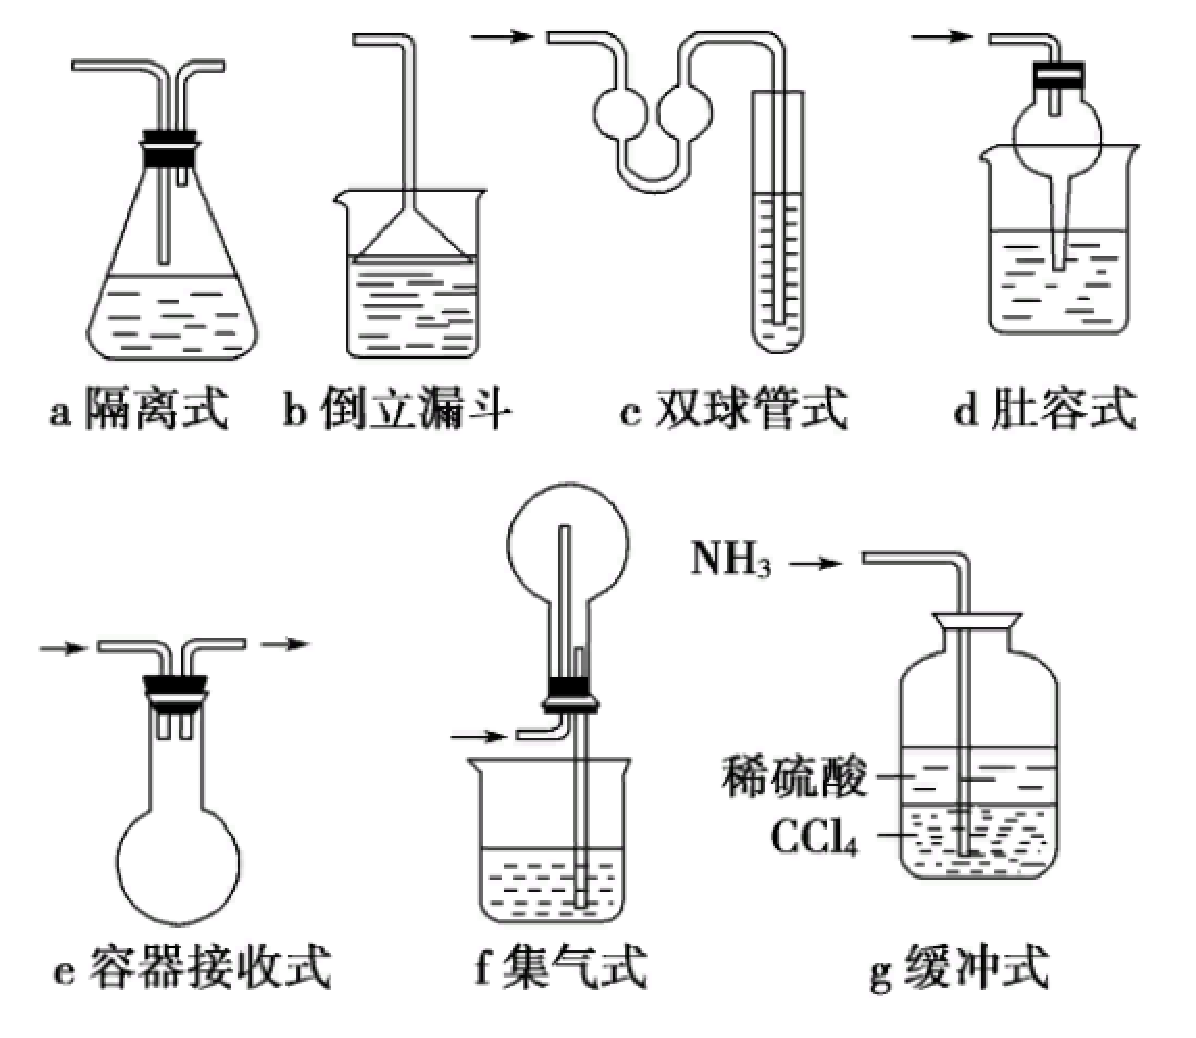
\includegraphics[scale=0.4]{res/Ammonia.pdf}
		\end{figure}
		\item 防污染
		\begin{itemize}
			\item 已取出的未用完的试剂一般不放回原瓶(块状固体如钠、钾等除外)
			\item 用胶头滴管滴加液体时,不伸入瓶内,不接触试管壁(向 \ce{FeSO4}溶液中加NaOH溶液制取 \ce{Fe(OH)2}除外)
			\item 取用试剂时试剂瓶盖倒放于桌面上
			\item 药匙和胶头滴管尽可能专用(或洗净、擦干后再取其他药品)
			\item 凡有污染性气体(如 \ce{Cl2}、 \ce{SO2}、 \ce{CO}、 \ce{NO_x}等)产生的实验均需对尾气进行处理
				\begin{itemize}
				\item 吸收(碱液吸收 \ce{Cl2}、 \ce{NOx},蘸 \ce{Na2CO3}溶液的棉花吸收 \ce{SO2})
				\item 点燃(用酒精灯点燃CO或将CO收集在气球中)
				\item 收集(用气球收集)
				\end{itemize}
			\end{itemize}
			\item 防堵塞:如高锰酸钾制取氧气
			\begin{figure}[h]
			 \centering
			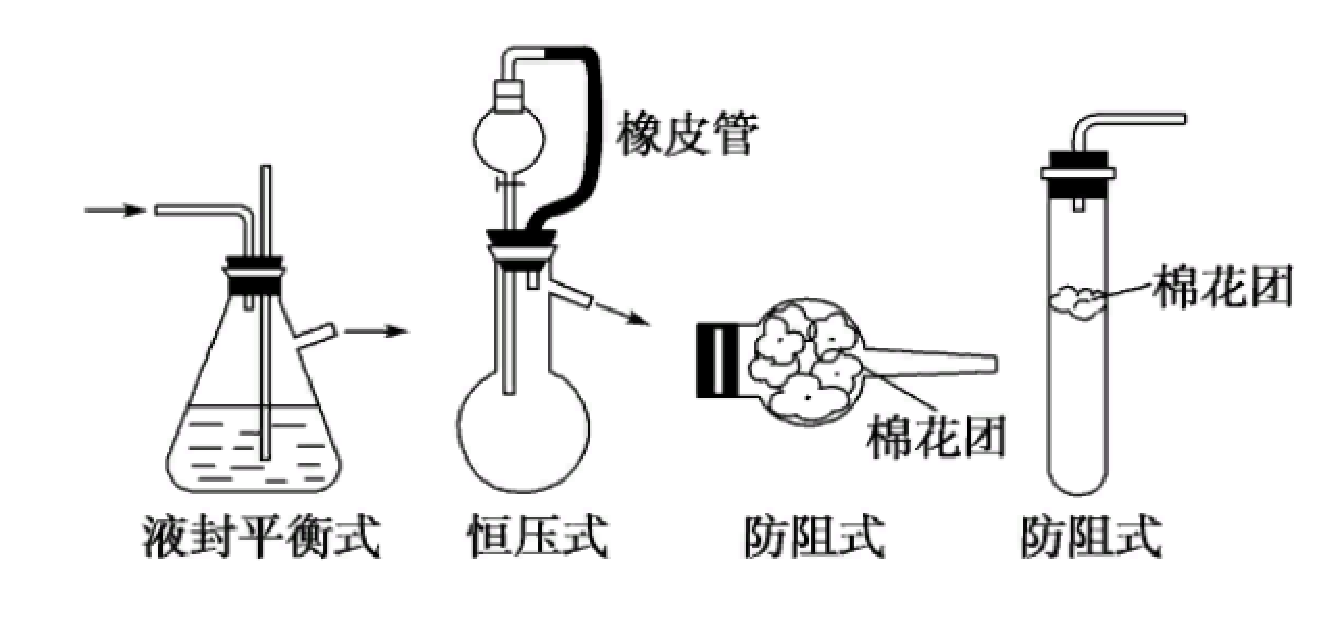
\includegraphics[scale=0.4]{res/Congestion.pdf}
			\end{figure}
	\end{itemize}
	
	
	
	\clearpage
	\section{物质的检验}
	
	
	\subsection{离子检验}
	
	\begin{center}
	\tablefirsthead{%
		\hline
		\textbf{离子} & \textbf{试剂和操作} & \textbf{现象} \\}
	\tablehead{%
		\hline
		\multicolumn{3}{|l|}{\small\sl 接上页}\\\hline
		\textbf{离子} & \textbf{试剂和操作} & \textbf{现象} \\
		}
	\tabletail{%
		\hline
		\multicolumn{3}{|r|}{\small\sl 接下页}\\
		\hline}
	\tablelasttail{\hline}

	\begin{supertabular}{|m{1cm}<{ \centering}|m{4cm}<{ \centering}|m{9cm}<{ \centering}|}
	\hline
	\multirow{2}{=}{ \centering \ce{I-}} & \ce{CCl4}、 \ce{Cl2} & 先无现象,加入 \ce{Cl2}后溶液呈紫色 \\ \cline{2-3} 
	~ & 稀 \ce{HNO3}、 \ce{AgNO3} & 产生黄色沉淀,不溶解 \\ \hline
	\multirow{2}{=}{ \centering \ce{Br-}} & \ce{CCl4}、 \ce{Cl2} & 先无现象,加入 \ce{Cl2}后溶液呈橙红色 \\ \cline{2-3} 
	~ & 稀 \ce{HNO3}、 \ce{AgNO3} & 产生淡黄色沉淀,不溶解 \\ \hline
	 \ce{Cl-} & 稀 \ce{HNO3}、 \ce{AgNO3} & 产生白色沉淀,不溶解 \\ \hline
	\multirow{3}{=}{ \centering \ce{Fe^3+}} & \ce{KSCN} & 溶液变为血红色 \\ \cline{2-3} 
	~ & \ce{K4[Fe(CN)6]} & 产生普鲁士蓝沉淀 \\ \cline{2-3} 
	~ & 苯酚 & 溶液变为紫色 \\ \hline
	\multirow{3}{=}{ \centering \ce{Fe^2+}} & \ce{KSCN}、 \ce{Cl2} & 溶液先无现象(排除 \ce{Fe^3+}),再变为血红色 \\ \cline{2-3} 
	~ & \ce{K3[Fe(CN)6]} & 产生滕氏蓝沉淀 \\ \cline{2-3} 
	~ & 酸性高锰酸钾溶液 & 溶液褪色 \\ \hline
	\multirow{2}{=}{ \centering \ce{NH4+}} & \multirow{2}{=}{ \centering 浓 \ce{NaOH}、加热、湿润红色石蕊试纸} & \multirow{2}{=}{ \centering 湿润红色石蕊试纸变蓝} \\
	& & \\ \hline
	\multirow{2}{=}{ \centering \ce{SO4^2-}} & \multirow{2}{=}{ \centering \ce{HCl}溶液、 \ce{BaCl2}溶液、稀 \ce{HNO3}} & \multirow{2}{=}{ \centering 先无现象(排除 \ce {Ag+}、 \ce {SO3^2-}),加入 \ce {HCl} 溶液后产生不溶白色沉淀,加入稀 \ce {HNO3} 无现象(排除 \ce {CO3^2-})} \\
	& & \\ \hline
	\multirow{2}{=}{ \centering \ce{CO3^2-}} & \multirow{2}{=}{ \centering \ce{CaCl2}溶液; \ce{HCl}溶液、澄清石灰水} & \multirow{2}{=}{ \centering 先产生白色沉淀(排除 \ce{HCO3-}),加入 \ce{CaCl2}溶液后产生无色无味气体(排除 \ce{SO3^2-}),使澄清石灰水浑浊} \\ 
	& & \\ \hline
	\multirow{2}{=}{ \centering \ce{SO3^2-}} & \multirow{2}{=}{ \centering \ce{BaCl2}溶液、 \ce{HCl}溶液、品红溶液} & \multirow{2}{=}{ \centering 先产生白色沉淀(排除 \ce{HSO3-}),加入 \ce{CaCl2}溶液后产生无色刺激性气体,使品红溶液褪色(排除 \ce{CO3^2-})} \\
	& & \\ \hline
	 \ce{Al^3+} & \ce{NaOH}溶液 & 先产生白色沉淀,一会溶解 \\ \hline
	 \ce{Cu^2+} & \ce{NaOH}溶液 & 产生蓝色沉淀,不溶解 \\ \hline
	 \ce{Ag+} & 稀硝酸、稀盐酸 & 产生白色沉淀,不溶解 \\ \hline
	 \ce{Ba+} & 稀硫酸、稀硝酸 & 产生白色沉淀,不溶解 \\ \hline
	 \ce{Na+} & \multicolumn{2}{c|}{用HCl清洗的洁净Pt丝蘸取溶液,酒精灯外焰加热,观察到黄色火焰} \\ \hline
	 \ce{K+} & \multicolumn{2}{c|}{用HCl清洗的洁净Pt丝蘸取溶液,酒精灯外焰加热,透过蓝色钴玻璃片观察到紫色火焰} \\
	\end{supertabular}
	\end{center}
	
	\subsubsection{焰色反应}
	\begin{itemize}
		% \item 锂盐:\textcolor[rgb]{0.698,0.149,0.098}{深红色}
		% \item 钠盐:\textcolor[rgb]{0.964,0.913,0.313}{黄色}
		% \item 钾盐:\textcolor[rgb]{0.882,0.741,0.858}{紫色}(透过蓝色钴玻璃)
		% \item 钙盐:\textcolor[rgb]{0.886,0.529,0.215}{砖红色}
		% \item 锶盐:\textcolor[rgb]{0.698,0.152,0.107}{洋红色}
		% \item 钡盐:\textcolor[rgb]{0.788,0.835,0.286}{黄绿色}
		% \item 铜盐:\textcolor[rgb]{0.537,0.8,0.262}{绿色}
		\item 钠盐:黄色
		\item 钾盐:紫色(透过蓝色钴玻璃观察)
	\end{itemize}
	\begin{figure}[h]
	 \centering
	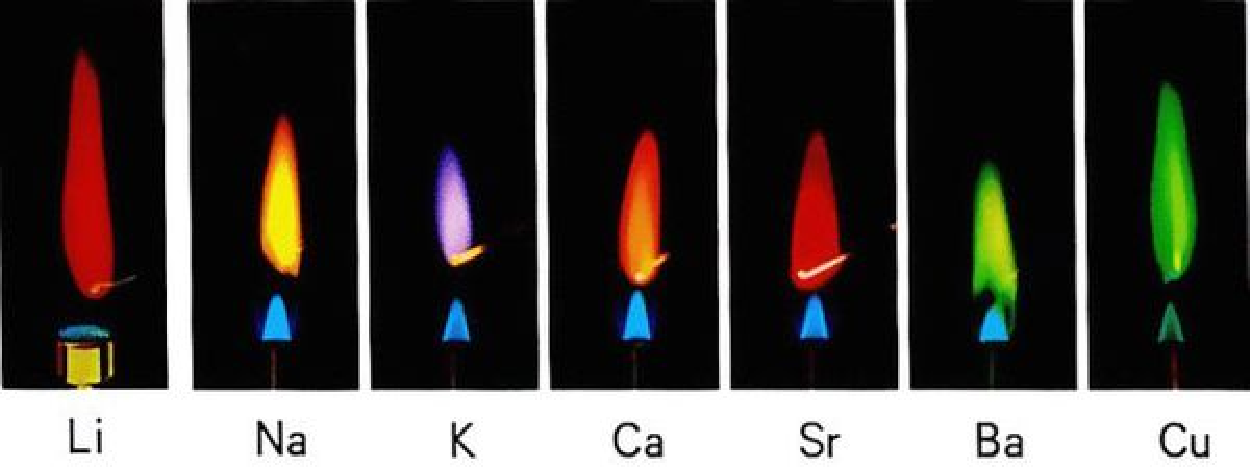
\includegraphics[scale=0.5]{res/FlameTest.pdf}
	\end{figure}
	
	
	\subsection{气体检验}
	
	\subsection{官能团检验}
	检验顺序:取样;醛基 > 碳碳双键
	\begin{itemize}
		\item 羧基:用碳酸氢钠溶液检验,放出气泡(二氧化碳)
		\item 羟基:用金属钠检验,放出气泡(氢气)
		\item 碳碳双键:
		\begin{itemize}
			\item 加入溴水(溴的四氯化碳溶液),溶液褪色
			\item 加入酸性高锰酸钾溶液,溶液褪色
		\end{itemize}
		\item 醛基:
		\begin{itemize}
			\item (碱化)滴加少量银氨溶液,水浴加热有银镜生成
			\item (碱化)滴加新制 \ce{Cu(OH)2}溶液,水浴加热产生砖红色沉淀
		\end{itemize}
		\item 卤原子: 先加碱溶液加热,然后冷却后加足量稀硝酸,滴入硝酸银溶液,产生沉淀
		\begin{itemize}
			\item 白色沉淀: \ce{Cl}
			\item 浅黄色沉淀: \ce{Br}
			\item 黄色沉淀: \ce{I}
		\end{itemize}
		\item 酯基:加碱加热,不分层
	\end{itemize}
	
	
	\clearpage
	\section{物质分离提纯}
	
	\begin{itemize}
		\item 物质的分离:
		\item 物质的提纯:
	\end{itemize}
	
	
	\subsection{物理法}
	
	\begin{itemize}
		\item 固体+固体
		\item \begin{itemize}
			\item 互溶:
			\item 不互溶:
		\end{itemize}
		\item 固体+液体
		\item \begin{itemize}
			\item 互溶:
			\item 不互溶:
		\end{itemize}
		\item 液体+液体
		\begin{itemize}
			\item 互溶:
			\item 不互溶:
		\end{itemize}
		\item 气体+气体:
		\begin{itemize}
			\item 洗气:
			\item 不互溶:
		\end{itemize}
	\end{itemize}
	
	\subsubsection{过滤}
	
	\paragraph{普通过滤(常压过滤)}
	
	一贴、二低、三靠
	
	\paragraph{热过滤}
	
	防止因温度下降而导致溶质结晶析出
	
	\paragraph{抽滤(减压过滤)}
	
	将固液较快彻底的分离。不适合过滤胶状沉淀或颗粒太小的沉淀
	
	\subsubsection{}
	
	\subsubsection{结晶}
	
	\paragraph{蒸发结晶}
	
	\subparagraph{操作注意事项}
	
	\begin{itemize}
		\item 当出现大量固体时,应停止加热
	\end{itemize}
	
	\subparagraph{使用范围}
	
	\begin{itemize}
		\item 单一溶质,溶质的溶解度随温度升高变化不大(或减小)、稳定
		\item 多种溶质,但目标
		\begin{itemize}
			\item 蒸发结晶、趁热过滤、洗涤、干燥
		\end{itemize}
	\end{itemize}
	
	\paragraph{冷却结晶}
	
	\begin{itemize}
		\item 原理:先加热溶液,配成热的饱和溶液,再通过
		\item 操作方法:蒸发浓缩、冷却过滤、
		\item 
	\end{itemize}
	
	\subparagraph{使用范围}
	
	\begin{itemize}
		\item 单一溶质,溶质不稳定,受热易分解(如结晶水合物、铵盐)
		\begin{itemize}
			\item 从 \ce{FeCl3}溶液中获取 \ce{FeCl3*H2O}
			\item 加入少量盐酸、蒸发浓缩、冷却结晶、
		\end{itemize}
		\item 多种溶质,目标溶质溶解度随温度升高而明显增大
	\end{itemize}
	
	\paragraph{重结晶}
	
	提纯
	
	溶解、加热浓缩、冷却结晶、(加活性炭脱色并趁热过滤)、过滤、洗涤、干燥
	
	使用范围:晶体与杂质
	
	\subsubsection{蒸馏}
	
	用蒸馏原理进行多次
	
	\paragraph{实验用品}
	
	蒸馏烧瓶、水冷
	
	\paragraph{操作注意事项}
	
	\begin{itemize}
		\item 先通水,再加热
		\item 刚开始手机到的馏份应弃去
		\item 全程控制好温度
	\end{itemize}
	
	\subsubsection{萃取分液}
	
	\paragraph{萃取条件}
	
	\begin{itemize}
		\item 萃取剂和原溶剂不相溶、密度不同
		\item 萃取物质在两种溶剂中溶解度不同
		\item 萃取剂和原溶质、原溶剂均不发生反应
	\end{itemize}
	
	\paragraph{萃取分液的操作步骤}
	
	\begin{enumerate}
		\item 碘水与 \ce{}	
	\end{enumerate}
	
	\paragraph{注意事项}
	
	\begin{itemize}
		\item 分液漏斗在洗涤干净后,必须检查上口和玻璃旋塞是否漏水。
		\item 充分震荡,适当放气,充分静置,
	\end{itemize}

	萃取后先将下层液体从分液漏斗中放出,再将上层液体从上口放出。注意使瓶塞上的凹槽对准小孔以平衡气压。
	
	\subsubsection{升华}
	
	在加热条件下分离出易升华的固体物质。
	
	\begin{itemize}
		\item \ce{NaCl}与 \ce{I2}的分离
		\item 精制砒霜
	\end{itemize}
	
	
	\subsubsection{渗析}
	
	\begin{center}
	\tablefirsthead{
		\hline
		\textbf{渗析} & \textbf{盐析} \\}
	\tablehead{
		\hline
		\multicolumn{2}{|l|}{\small\sl 接上页}\\\hline
		\textbf{渗析} & \textbf{盐析} \\
		}
	\tabletail{
		\hline
		\multicolumn{2}{|r|}{\small\sl 接下页}\\
		\hline}
	\tablelasttail{\hline}
	\begin{supertabular}{|m{0.5\textwidth}<{ \centering}|m{0.5\textwidth}<{ \centering}|}
		\hline
		& \\ \hline
		& \\
	\end{supertabular}
	\end{center}
	
	
	\subsection{化学法}
	
	\paragraph{四原则}
	
	\begin{itemize}
		\item 不增
		\item 不减
		\item 易分离
		\item 易复原
	\end{itemize}
	
	\paragraph{四必须}
	
	\begin{itemize}
		\item 除杂试剂必须过量
		\item 
	\end{itemize}
	
	\subsubsection{常见混合物气体除杂}
	
	\begin{center}
	\tablefirsthead{
		\hline
		\textbf{混合物} & \textbf{杂质} & \textbf{除杂试剂} & \textbf{主要操作} \\}
	\tablehead{
		\hline
		\multicolumn{4}{|l|}{\small\sl 接上页}\\\hline
		\textbf{混合物} & \textbf{杂质} & \textbf{除杂试剂} & \textbf{主要操作} \\
		}
	\tabletail{
		\hline
		\multicolumn{4}{|r|}{\small\sl 接下页}\\
		\hline}
	\tablelasttail{\hline}
	\begin{supertabular}{|m{2cm}<{ \centering}|m{1cm}<{ \centering}|m{5cm}<{ \centering}|m{5cm}<{ \centering}|}
		\hline
		& & & \\
	\end{supertabular}
	\end{center}
	
	\subsubsection{常见混合物固体除杂}
	
	\begin{center}
	\tablefirsthead{
		\hline
		\textbf{混合物} & \textbf{杂质} & \textbf{除杂试剂} & \textbf{主要操作} \\}
	\tablehead{
		\hline
		\multicolumn{4}{|l|}{\small\sl 接上页}\\\hline
		\textbf{混合物} & \textbf{杂质} & \textbf{除杂试剂} & \textbf{主要操作} \\
		}
	\tabletail{
		\hline
		\multicolumn{4}{|r|}{\small\sl 接下页}\\
		\hline}
	\tablelasttail{\hline}
	\begin{supertabular}{|m{2cm}<{ \centering}|m{1cm}<{ \centering}|m{5cm}<{ \centering}|m{5cm}<{ \centering}|}
		\hline
		碳粉 & \ce{CuO} & 足量稀盐酸 & 过滤 \\ \hline
		 \ce{Fe2O3} & \ce{Al2O3} & 足量稀盐酸 & 过滤 \\ \hline
		碳粉 & \ce{CuO} & 足量稀盐酸 & 过滤 \\ \hline
		碳粉 & \ce{CuO} & 足量稀盐酸 & 过滤 \\ \hline
		碳粉 & \ce{CuO} & 足量稀盐酸 & 过滤 \\ \hline
		碳粉 & \ce{CuO} & 足量稀盐酸 & 过滤 \\ \hline
	\end{supertabular}
	\end{center}
	
	\subsubsection{常见混合物溶液除杂}
	
	\begin{center}
	\tablefirsthead{
		\hline
		\textbf{混合物} & \textbf{杂质} & \textbf{除杂试剂} & \textbf{主要操作} \\}
	\tablehead{
		\hline
		\multicolumn{4}{|l|}{\small\sl 接上页}\\\hline
		\textbf{混合物} & \textbf{杂质} & \textbf{除杂试剂} & \textbf{主要操作} \\
		}
	\tabletail{
		\hline
		\multicolumn{4}{|r|}{\small\sl 接下页}\\
		\hline}
	\tablelasttail{\hline}
	\begin{supertabular}{|m{2cm}<{ \centering}|m{1cm}<{ \centering}|m{5cm}<{ \centering}|m{5cm}<{ \centering}|}
		\hline
		 \ce{NaHCO3}溶液 & \ce{Na2CO3} & \ce{CO2} & 通入气体 \\ \hline
		 \ce{FeCl3}溶液 & \ce{FeCl2} & \ce{Cl2} & 通入气体 \\ \hline
		 \ce{FeCl2}溶液 & \ce{FeCl3} & \ce{Fe} & 通入气体 \\ \hline
		 \ce{CuCl2}溶液 & \ce{FeCl3} & \ce{CuO}或 \ce{Cu(OH)2} & 过滤 \\ \hline
		乙酸乙酯 & 乙酸 & 饱和 \ce{Na2CO3}溶液 & 分液 \\ \hline
	\end{supertabular}
	\end{center}

	
	\subsubsection{沉淀法}
	\paragraph{ \ce{Al2O3}和 \ce{MgO}固体}
	\begin{enumerate}
		\item \ce{NaOH}溶液:过滤得 \ce{Al()}和 \ce{MgO}固体
		\item 稀 \ce{HCl}:得氢氧化铝
		\item 加热氢氧化铝:得氧化铝
	\end{enumerate}
	\paragraph{ \ce{Fe2O3}和 \ce{SiO2}固体}
	\begin{enumerate}
		\item 稀 \ce{HCl}:得 \ce{FeCl3}溶液和 \ce{SiO2}固体
		\item \ce{NaOH}溶液:得 \ce{Fe(OH)3}沉淀
		\item 加热氢氧化铝:得氧化铝
	\end{enumerate}
	\paragraph{ \ce{AlCl3}和 \ce{FeCl3}的混合溶液}
	\begin{enumerate}
		\item \ce{NaOH}溶液:得 \ce{Fe(OH)3}沉淀和 \ce{AlCl3}溶液
		\item 稀 \ce{HCl}:得 \ce{FeCl3}溶液
	\end{enumerate}
	
	\subsubsection{气化法}
	
	\subsubsection{杂质转换法}
	
	\subsubsection{酸碱溶解法}
	
	\subsubsection{氧化还原法}
	
	\subsubsection{加热分解法}
		
	\subsubsection{调节pH法}
	
	\subsubsection{电解法}
	
	粗金属作阳极,纯金属作阴极
	
\end{document}